\section{Ground Heat Transfer Calculations using Foundation:Kiva}

Kiva\textsuperscript{TM} is an open source foundation heat transfer
calculation tool developed by Big Ladder Software.

\url{http://bigladdersoftware.com/projects/kiva/}

Kiva is the product of Neal Kruis's dissertation where he demonstrated
that accurate foundation heat transfer calculations can be performed
quickly (on the order of 5 seconds) without any noticeable loss of
accuracy relative to a mesh-independent, fully three-dimensional
simulation.

\subsection{Approach}

Within EnergyPlus, Kiva is used to perform two-dimensional finite
difference heat transfer calculations. Each foundation is represented by
a single floor and wall in Kiva, meaning that individual walls in
EnergyPlus are mapped to a single representative wall in the
two-dimensional context using an area weighted average for any
non-uniform boundary conditions among the walls.

Kiva uses the boundary conditions from EnergyPlus:

\begin{itemize}
\tightlist
\item
  weather data,
\item
  solar position, and
\item
  zone temperatures (from previous timestep),
\item
  zone radiation (solar, IR, etc.)
\end{itemize}

to calculate the resulting convective heat gains and surface
temperatures for the floor and wall surfaces associated with a single
Foundation:Kiva object. Because Kiva performs multi-dimensional finite
difference calculations, the associated surfaces do not use the same
HeatBalanceAlgorithm (e.g., Conduction Transfer Functions) as the rest
of the model.

\subsection{Two-dimensional
Approximation}

The two-dimensional approximation method employed by Kiva relies on
knowing the footprint shape, area, and exposed perimeter of each
instance. The appropriate footprint shape, area, and exposed perimeter
for each instance will be defined within the context of the overall
geometry of the Foundation surfaces.

The general method is to define the width of the floor (the distance
from the symmetry plane to the wall interior),\(w\) in the
two-dimensional context as:

\begin{equation}
A/P_{exp}
\end{equation}

where \(A\) is the area of the foundation footprint, and \(P_{exp}\) is
the exposed perimeter of the foundation (See
SurfaceProperty:ExposedFoundationPerimeter).

Kiva also has the capability to adjust this width to account for concave
foundation footprint shapes (Note: this also relies on detailed input of
the exposed foundation perimeter for each segment of the footprint
polygon). This adjustment is based on the boundary layer adjustment
method described by Kruis and Krarti (2017). The approach adjusts the
exposed perimeter to account for interactions in heat flow within
concave corners and narrow gaps between two exposed edges.

This approach allows for accurate representation of building foundation
heat transfer without performing three-dimensional calculations. Because
the two-dimensional context is symmetric, the domain can be divided in
half to further reduce the number of calculations.

\subsection{Numerical Calculations}

Kiva automatically discretizes the two-dimensional domain into
rectangular cells. The size of each cell is defined by the
Foundation:Kiva:Settings object's ``Minimum Cell Dimension'' and
``Maximum Cell Growth Coefficient''. The ``Minimum Cell Dimension''
defines the smallest possible dimension of a cell within the domain.
Cells along a block boundary start at this size and grow geometrically
away from the boundary according to the ``Maximum Cell Growth
Coefficient''. This is evident from Figures \ref{fig:ms} and
\ref{fig:mb} which show the discretization for a single foundation at
close and far perspectives, respectively.

\begin{figure}
\centering
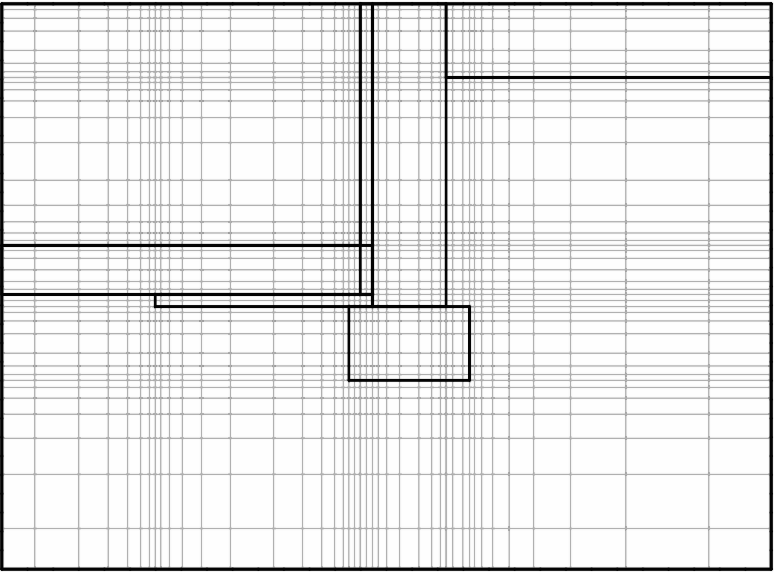
\includegraphics{media/kiva-2d-mesh.png}
\caption{Example generated discretization near foundation
perimeter\label{fig:ms}}
\end{figure}

\begin{figure}
\centering
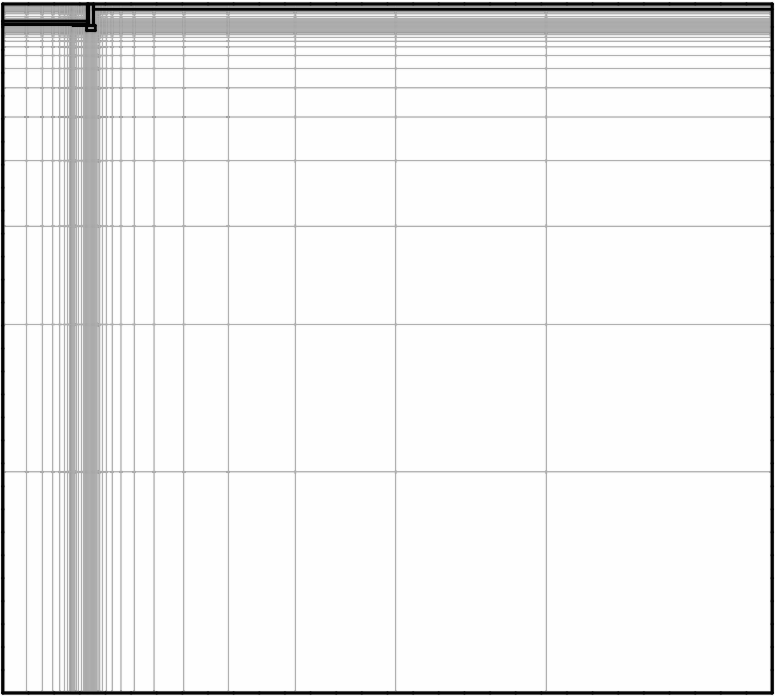
\includegraphics{media/kiva-2d-mesh-big.png}
\caption{Example generated discretization of full domain\label{fig:mb}}
\end{figure}

The discretized partial differential equations are solved using the
Alternating Direction Implicit (ADI) finite difference time stepping
scheme. This scheme provides relatively fast calculations with stable
results as demonstrated by Kruis and Krarti (2015).

\subsection{Boundary Conditions}

\begin{figure}
\centering
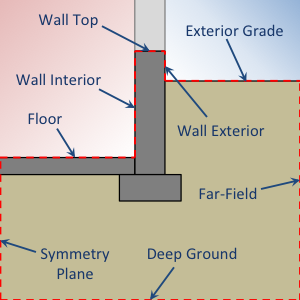
\includegraphics{media/kiva-2d-boundaries.png}
\caption{Boundary conditions in Kiva's two-dimensional
context\label{fig:bnd}}
\end{figure}

\textbf{Symmetry Plane:} Zero heat flux in the horizontal direction.

\textbf{Wall Top:} Zero heat flux in the vertical direction (assumes
heat transfer through the exterior wall above is one-dimensional in the
horizontal direction).

\textbf{Deep Ground:} Either constant temperature or zero vertical heat
flux, depending on user input. Deep ground depth may be automatically
calculated based on water table estimates using a method defined by
Williams and Williamson (1989).

\textbf{Far-Field:} Zero heat flux in the horizontal direction. If this
boundary is sufficiently far from the building, this will result in an
undisturbed ground temperature profile.

\textbf{Interior Surfaces:}

\begin{itemize}
\tightlist
\item
  Convection is calculated according to the TARP method (see
  SurfaceConvectionAlgorithm:Inside).
\item
  Long and short wave radiation is passed from EnergyPlus radiant
  exchange and interior solar distribution algorithms. Note: Kiva uses
  area weighted averages to define the radiation incident on walls in
  the two-dimensional context.
\end{itemize}

\textbf{Exterior Surfaces:}

\begin{itemize}
\tightlist
\item
  Convection is calculated according to the DOE-2 method (see
  SurfaceConvectionAlgorithm:Outside). Wind speeds along the exterior
  grade are calculated at the roughness height.
\item
  Exterior long wave radiation is calculated using the same algorithms
  used for other EnergyPlus surfaces. Note: there is no explicit radiant
  exchange between the ground and building surfaces.
\item
  Exterior solar incidence is uniform along the exterior grade surfaces.
  No shading is taken into account. Solar incidence along the wall
  exterior
\end{itemize}

\subsection{Multiple Kiva Instances}

In some cases, a single Foundation boundary condition might require
multiple Kiva instances:

\textbf{Multiple Zones:} If the surfaces in several zones reference the
same Foundation:Kiva object, each zone will be calculated using separate
Kiva instances.

\textbf{Walk-Out Basements:} Walkout basements are defined by using
walls of different heights all referencing the same Foundation:Kiva
object.

\begin{figure}
\centering
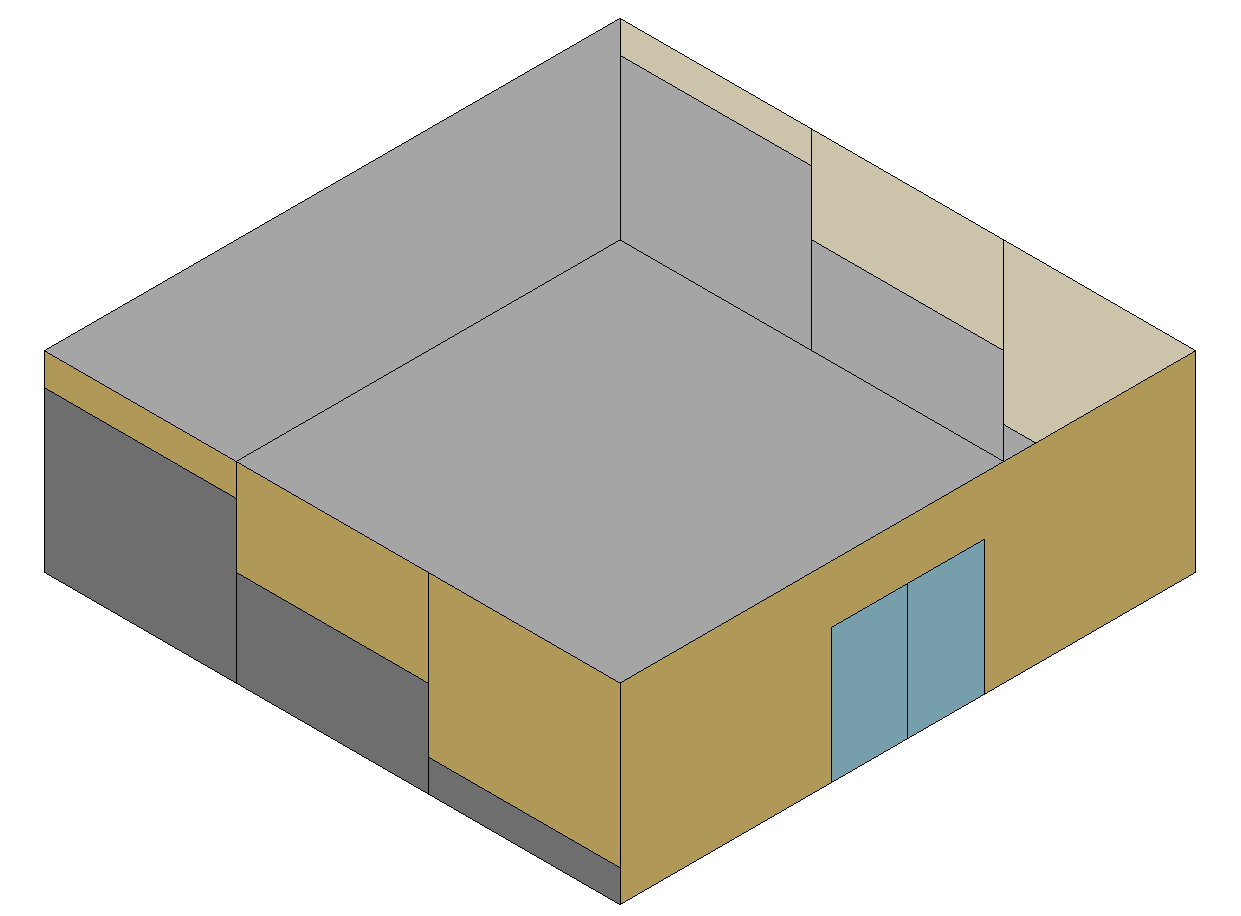
\includegraphics{media/kiva-walkout-segs.png}
\caption{Walkout basement surfaces (in gray) all reference the same
Foundation:Kiva object\label{fig:wo-s2}}
\end{figure}

A separate Kiva instance will be run for any walls with different
heights associated with the same Foundation:Kiva object. Figure
\ref{fig:wo-s2} shows how the grouping of walls by height based on the
basement in Figure \ref{fig:wo-w}, including the portion that is only a
slab.

\begin{figure}
\centering
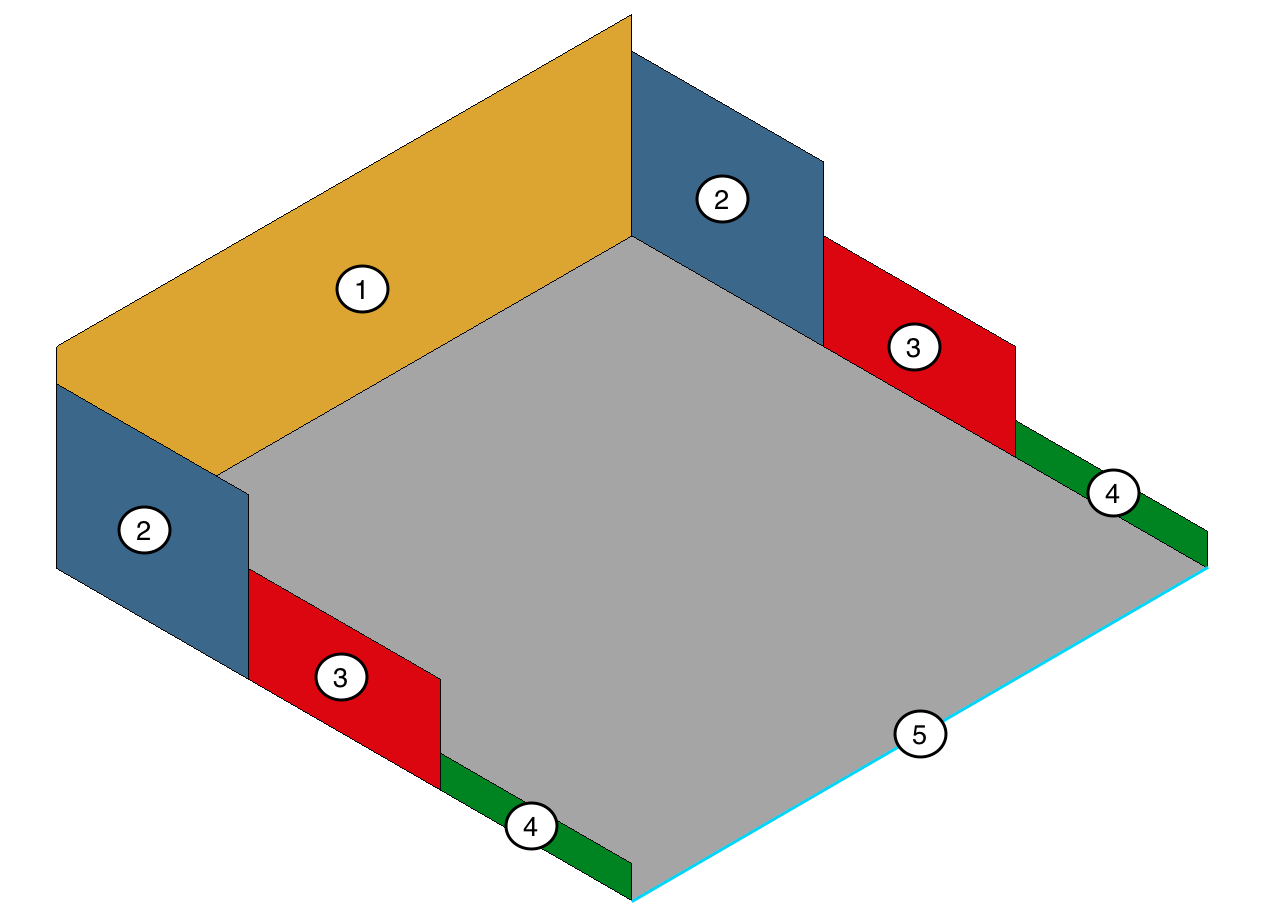
\includegraphics{media/kiva-walkout-walls.png}
\caption{Walkout basement Kiva instances (one for each wall
height)\label{fig:wo-w}}
\end{figure}

The resulting five two-dimensional contexts will look like Figures
\ref{fig:wo-1} - \ref{fig:wo-5}.

\begin{figure}
\centering
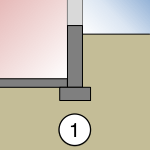
\includegraphics{media/kiva-walkout-2d-1.png}
\caption{Group 1 Kiva context\label{fig:wo-1}}
\end{figure}

\begin{figure}
\centering
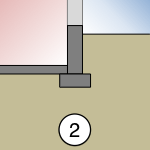
\includegraphics{media/kiva-walkout-2d-2.png}
\caption{Group 2 Kiva context\label{fig:wo-2}}
\end{figure}

\begin{figure}
\centering
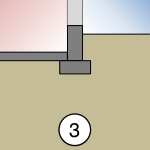
\includegraphics{media/kiva-walkout-2d-3.png}
\caption{Group 3 Kiva context\label{fig:wo-3}}
\end{figure}

\begin{figure}
\centering
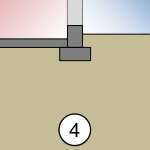
\includegraphics{media/kiva-walkout-2d-4.png}
\caption{Group 4 Kiva context\label{fig:wo-4}}
\end{figure}

\begin{figure}
\centering
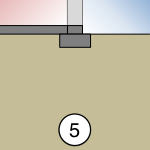
\includegraphics{media/kiva-walkout-2d-5.png}
\caption{Group 5 Kiva context\label{fig:wo-5}}
\end{figure}

Each Kiva instance with a different wall height will calculate different
heat fluxes, convective coefficients and surface temperatures for both
the wall and the floor. The heat flux through the associated floor will
be weighted according to the fraction of the total exposed perimeter,
\(P_{exp,tot}\), represented by each segment of different height. The
total heat flux through the walkout basement floor is:

\begin{equation}
\dot{q} = \sum^{N_{segs}}_i{\frac{P_{exp,i}}{P_{exp,tot}}}\cdot h_i \left(T_\infty - T_{floor,i} \right)
\end{equation}

The weighted average convective coefficient for the walkout basement
floor surface is:

\begin{equation}
\bar{h} = \sum^{N_{wall,segs}}_i{\frac{P_{exp,i}}{P_{exp,tot}}}\cdot h_i
\end{equation}

The weighted average temperature for the floor surface is:

\begin{equation}
\bar{T}_{floor} = T_\infty - \dot{q}/\bar{h}
\end{equation}

\textbf{Multiple Floor Surfaces:} If a floor has multiple constructions
(e.g., carpeted and bare) each surface must reference a separate
Foundation:Kiva object, or be combined into a single equivalent
construction.

\subsection{Core Zone Slabs}

Because core zones have no exposed perimeter, they are assumed to
exchange heat only with the deep ground boundary condition. This is
calculated using a one-dimensional finite difference formulation. The
associated Kiva instance will use only the description of the slab and
the deep ground boundary condition to define the heat flux through the
surface.

\begin{figure}
\centering
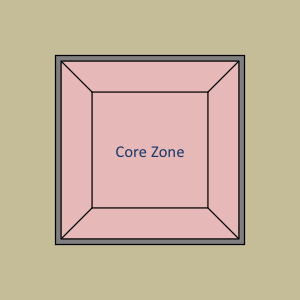
\includegraphics{media/kiva-core-zone.png}
\caption{Core zone (no exposed perimeter)\label{fig:cz}}
\end{figure}

\begin{figure}
\centering
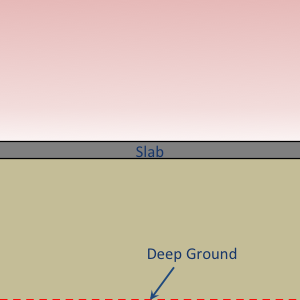
\includegraphics{media/kiva-core-zone-1d.png}
\caption{Core zone one-dimensional context\label{fig:cz-1}}
\end{figure}

\subsection{Warm-Up}

The traditional ``warm-up'' period in EnergyPlus (of repeating a single
day) presents several challenges for foundation heat transfer
calculations:

\begin{itemize}
\tightlist
\item
  As the ground can have time constants on the order of years, a single
  day is simply not long enough to adequately capture the thermal
  history of the ground.
\item
  Any repetition of a single day would erase any pre-calculated thermal
  history and likely take much longer to converge.
\end{itemize}

Instead, Kiva instances are initialized independently from the rest of the simulation using the accelerated initialization method developed by Kruis (2015). This method looks back in the weather file and simulates long timestep (on the order of weeks or months) calculations using an implicit numerical scheme. These long timesteps allow Kiva to capture a long term history of the ground without running the entire building model.

The initialization of the ground relies on assumptions of indoor air temperatures (as they are not yet calculated by EnergyPlus). When a thermostat is assigned to a zone with Kiva foundation surfaces, the assumed temperature is equal to the setpoint (or a weighted average of heating and cooling setpoints depending on outdoor temperature). For zones without thermostats, a constant 22 \textsuperscript{o}C indoor temperature is assumed.

\subsection{Validation}

Kiva has been tested against the BESTEST Ground coupled cases with
accuracy within 3\% of the reference solutions (Kruis and Krarti, 2015).

\subsection{References}

{[}1{]} N. Kruis and M. Krarti, ``Kiva\textsuperscript{TM}: A Numerical
Framework for Improving Foundation Heat Transfer Calculations,'' Journal
of Building Performance Simulation, vol.~8, no. 6, pp.~449-468, 2015.

{[}2{]} N. Kruis, ``Development and Application of a Numerical Framework for Improving Building Foundation Heat Transfer Calculations,''
Ph.D. Dissertation. University of Colorado, 2015.

{[}3{]} N. Kruis and M. Krarti, ``Three-dimensional accuracy with
two-dimensional computation speed: using the Kiva\textsuperscript{TM}
numerical framework to improve foundation heat transfer calculations,''
Journal of Building Performance Simulation, vol.~10, no. 2, pp.~161?182,
2017.

{[}4{]} T. Williams and A. Williamson, ``Estimating Water-Table
Altitudes for Regional Ground-Water Flow Modeling, U.S. Gulf Coast,''
Ground Water, vol.~27, no. 3, pp.~333-340, 1989.
